\subsection{Evaluating Models} \label{evalmodels}
%\todo{shorten this}
To compare the performance of different model predictions, we calculated the \textit{accuracy} of each model as
\begin{equation}
    \text{accuracy} = \frac{tp+tn}{tp+tn+fp+fn},
\end{equation}
where $tp$ and $tn$ are true positives and true negatives, and $fp$ and $fn$ are false positives and false negatives respectively. Additionally, detailed confusion matrices are also reported. %\cite{vanwinckelen2012estimating}. 

%\sophie{should figures 2 and 3 be kept?}
%\denes{No, but we could report all the confusion matrices for each model (possibly in the appendices).}
To get a more balanced idea about model performance, we also compute F1 scores as:
%Precision is defined as the proportion of true positives to the total number of predictions predicted positive, and is a percentage of returned results which are relevant. Recall is defined to be the proportion of true positives to the total number of actual positives, and is a percentage of relevant data which have been correctly classified \cite{buckland1994relationship}.
\begin{equation}
\begin{aligned}
    \text{precision} = \frac{tp}{tp+fp} \quad
 \text{recall} = \frac{tp}{tp+fn}\\
 \vspace{0.1cm}\\
F1 = \frac{2\times\text{precision} \times \text{recall}}{\text{precision} + \text{recall}},
\end{aligned}
\end{equation}
which is effectively an F measure with $\beta=1$ \cite{sokolova2006beyond}.
%Both metrics are important to take into consideration, and ultimately we use the F1 measure, which can be interpreted as the harmonic mean between precision and recall \cite{buckland1994relationship}, and accuracy score for evaluation of each classifier.

% An issue associated with training models is the possibility for the model to \textit{overfit}.
To avoid over-fitting, we use 5-fold cross validation. The whole dataset was split in a training:validation:test set in a 18:72:10 ratio. 10\% of the original dataset was kept as a test set to validate hyperparameter tuning. The remaining 90\%, the data was split in an 80:20 ratio for the 5-fold training; 80\% was used to train the model, the 20\% was used to optimize hyperparamters. %The model trains on the training set, and the validation set is used for optimising the hyperparameters of the model.
%Overfitting occurs when a model captures unwanted bias and noise in the data that it negatively impacts the performance of a model. The model corresponds to it's initial training data too well, and fails to predict unseen data reliably. In order to limit overfitting, a popular re-sampling technique called $k$-fold cross validation is used.
%In cross validation, the dataset is split into $k$ random subsets, known as folds, and one is selected as a test set for the model to test on, while the others are used as a training set for the model to train on. This is repeated $k$ times where a different subset of data is used as the test set each time, and the overall performance of the model is calculated as the average of accuracy scores for each iteration \cite{berrar2019cross}.

\subsection{Hyperparameter Tuning} \label{hpt}
We used a brute-force grid search to fine tune parameters of the model that are outside the usual training domain (hyperparameters) e.g. the number of trees in a random forest classifier.
%For each model, the \textit{hyperparameters}, parameters that are not optimised by the training algorithm e.g. the number of trees in a random forest classifier, were tuned manually by using a grid search to test different values.
%A grid search uses brute force to search the entire space for different hyperparameter configurations.
The best combination of hyperparameters for a model is determined by whichever has the highest accuracy on the validation set using 5-fold cross validation.

For logistic regression, the type of solver, penalty function and the $C$  terms value were adjusted. $C$ is a regularisation term; 
%\textit{Regularisation} prevents overfitting of training data by penalising large weights when training a logistic regression predictor, and the parameter $C$ mentioned is used to control the effect of this\cite{ahmadian1998regularisation}. 
the lower the value of $C$, the stronger the effect of regularisation. We found that  $C=1.0$, and a `liblinear' solver resulted in the best average accuracy.

$l1$ regularisation penalises the sum of absolute values of weights, whereas $l2$ regularisation penalises the sum of squares of the weights \cite{ahmadian1998regularisation}. For our data, $l2$ regularisation was gave the best results (\figref{lrlc}) \denes{Could we plot l1 vs l2 here? That would be quite convincing}.

\begin{figure}[ht]
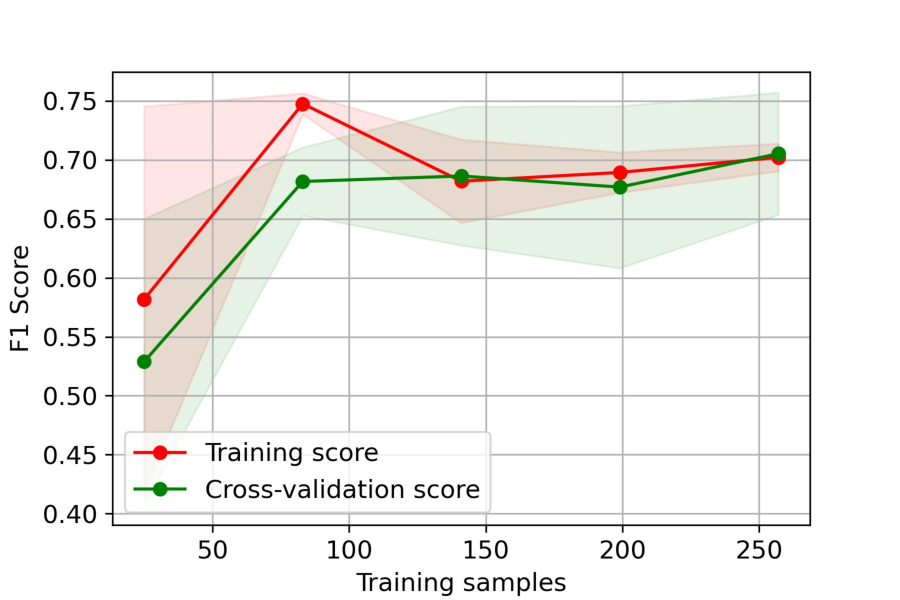
\includegraphics[width=8.5cm]{plots/LR TVT LC F1.pdf}
\caption{Logistic Regression Learning Curve}
\label{fig:lrlc}
\centering
\end{figure}

\begin{figure}[ht]
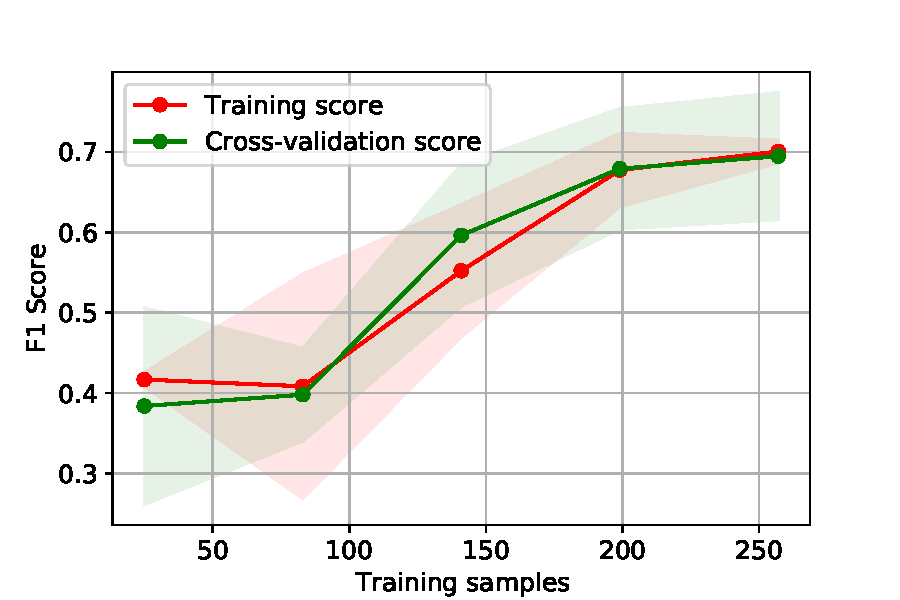
\includegraphics[width=8.5cm]{plots/SVM TVT LC F1.pdf}
\caption{Linear SVM Learning Curve \denes{consider subplots with logistic learning curve}}
\vspace{-0.5em}
\label{svmlc}
\centering
\end{figure}

For SVMs, the two main hyperparameters that were adjusted were the kernel type and penalty value $C$. Using a linear kernel and and $C=0.2$ gave the highest F1 score on the test set compared to other kernels. The learning curve for an SVM model using a linear kernel is shown in Figure \ref{svmlc}.

\section{Experimental Results} \label{experresults}
Our main results are reported in Table~\ref{results} and \figref{confusionmatricesr2}.
%The test set is completely left out from the training process of the model, and is only used during evaluation. This is to see how well models generalise to unseen data which replicate new match data, as the test set is never used before evaluation. During evaluation, all other data is used for training the model (training and validation).
Both accuracy and F1 score are reported for the validation and test sets. The standard deviation\todo{?} for each score for the validation set is reported as a basis of defining uncertainty. The validation column shows that most models perform comparably with approx. 70\% accuracy (and also with comparable F1 score). MLP Neural Networks slightly over-perform their competitors, but the difference is not significant.
\todo{can we report Standard Error in the Mean instead? that is standard deviation divided by root(N), or just divided by root(5) as N=5 here I think}.
For the MLP, we used a  \textit{relu} activation function.
%This function returns $f(x) = \max{(0,x)}$ and defines the output of a node in a hidden layer given a set of inputs. 
The hidden layer size was set to 2 and the maximum number of iterations the solver iterates was chosen to be 200. The solver for weight optimization is set to `lbfgs', a quasi-Newton optimizer. The learning rate for scheduling weight updates is set to constant; more detail on different hyperparameters can be found in Scikit Learns documentation \cite{pedregosa2011scikit}. However, the generic layered structure of a neural network has proven to be time consuming. Additionally, this technique is considered a ``black box'' technology, and finding out why a neural network has poor performance, or how it performs the classification process, is extremely difficult \cite{noriega2005multilayer}.

On the test set (following hyperparameter tuning) it seems that Logistic regression is performing noticeably better than other models. One interesting thing we noticed was how most models did not perform noticeably better after hyperparameter tuning -- with logistic regression being an exception to this.

\begin{table}[H]
\caption{Model performance comparing validation and test sets}
\label{results}
\centering
\setlength{\tabcolsep}{3pt}
\scalebox{1.05}{%
\begin{tabular}{ l|c c|c c }

\multirow{2}{4em}{Model} &
\multicolumn{2}{|c|}{Validation set} &
\multicolumn{2}{|c}{Test set} \\
\cline{2-5}
  & Acc & F1 & Acc & F1 \\

\hline \hline 
Logistic Regression & 0.699$\pm{0.053}$ & 0.705$\pm{0.052}$ & 0.722 & 0.706 \\
Random Forest & 0.677$\pm{0.071}$ & 0.688$\pm{0.073}$ & 0.667 & 0.684 \\
Support Vector Machine & & \\
$\rightarrow$ Linear & 0.696$\pm{0.064}$ & 0.690$\pm{0.078}$ & 0.639 & 0.629 \\
$\rightarrow$ RBF    & 0.700$\pm{0.056}$ & 0.677$\pm{0.077}$ & 0.667 & 0.600 \\
$\rightarrow$ Polynomial & 0.705$\pm{0.046}$ & 0.685$\pm{0.046}$ & 0.611 & 0.563\\
$\rightarrow$ Sigmoid & 0.705$\pm{0.039}$ & 0.690$\pm{0.041}$ & 0.694 & 0.621 \\
MLP Neural Network & 0.696$\pm{0.043}$ & 0.708$\pm{0.045}$ & 0.694 & 0.703\\
[1ex]
\hline
\end{tabular}}
\end{table}

Receiving operating characteristics (ROC) learning curves and the trade-off between precision and recall can be seen from Figs.~\ref{fig:roc}~and~\ref{fig:par}.
\denes{Once these are replotted on single plots, we could try to comment on whether there is a noticeable difference}.
%ROC curves demonstrate the performance of a classification model for all classification thresholds. The closer the apex of the curve is to the upper left hand corner, the greater the model's discriminatory ability \cite{fan2006understanding}. This is plotted for each type of classifier, including the SVM model using a linear kernel. 
For each trained model, we use it's accuracy score, F1 measure and the area under its ROC curve to evaluate overall performance\denes{do we report area aswell anywhere?}.

\begin{figure}[ht]
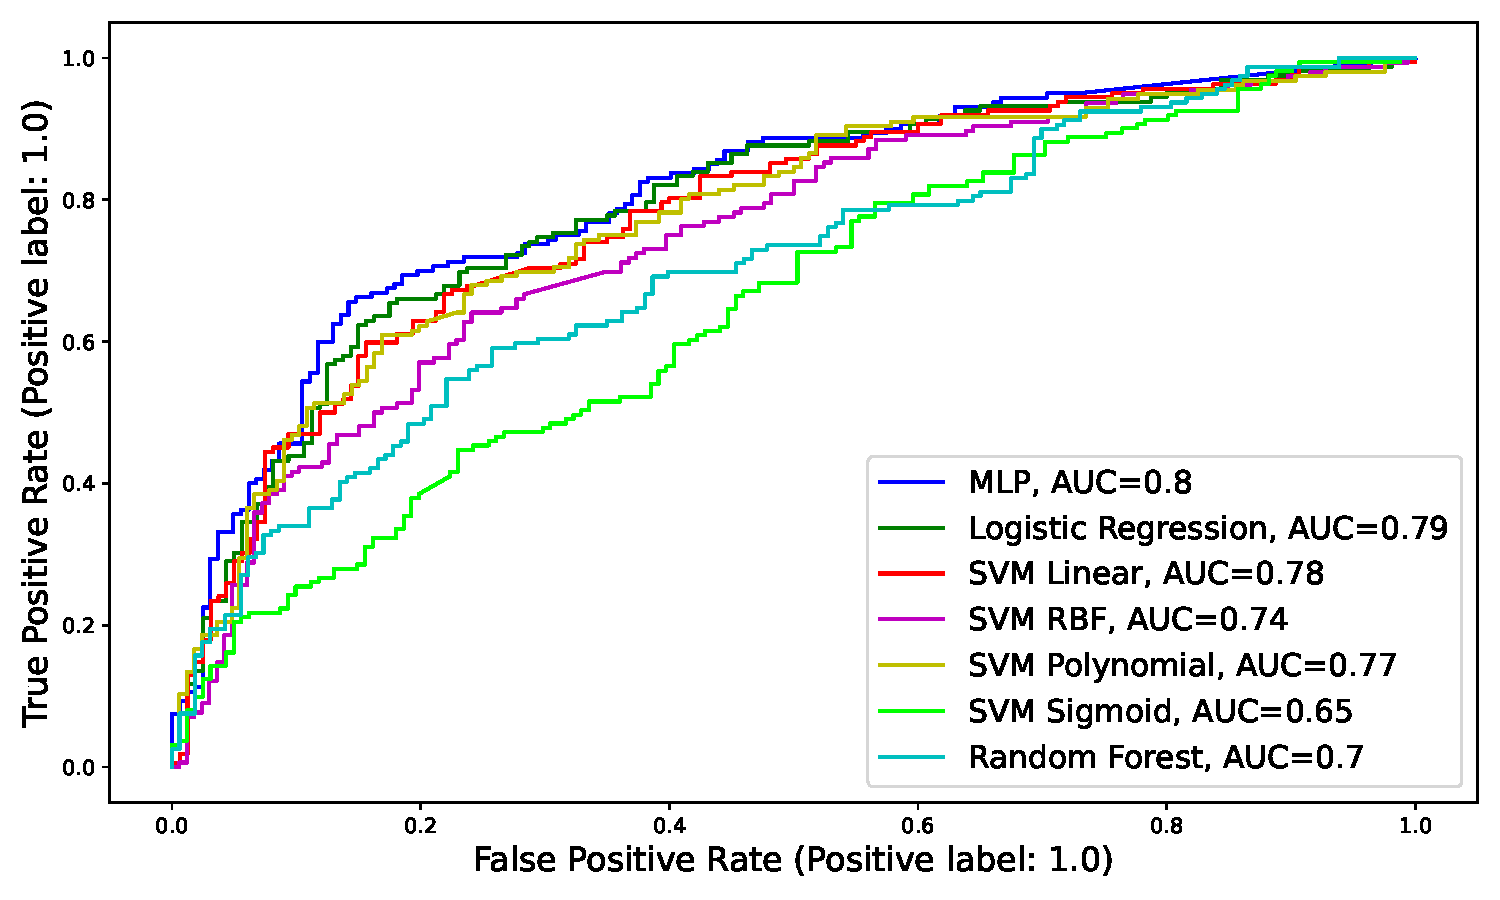
\includegraphics[width=8.5cm]{plots/roccurves.pdf}
\caption{ROC Learning Curves.}
%\denes{As discussed, please replot without axis / bigger fonts. Or actually, why not do one single ROC plot (you have 4 colours anyway?}}

\label{fig:roc}
\centering
\end{figure}

\begin{figure}[ht]
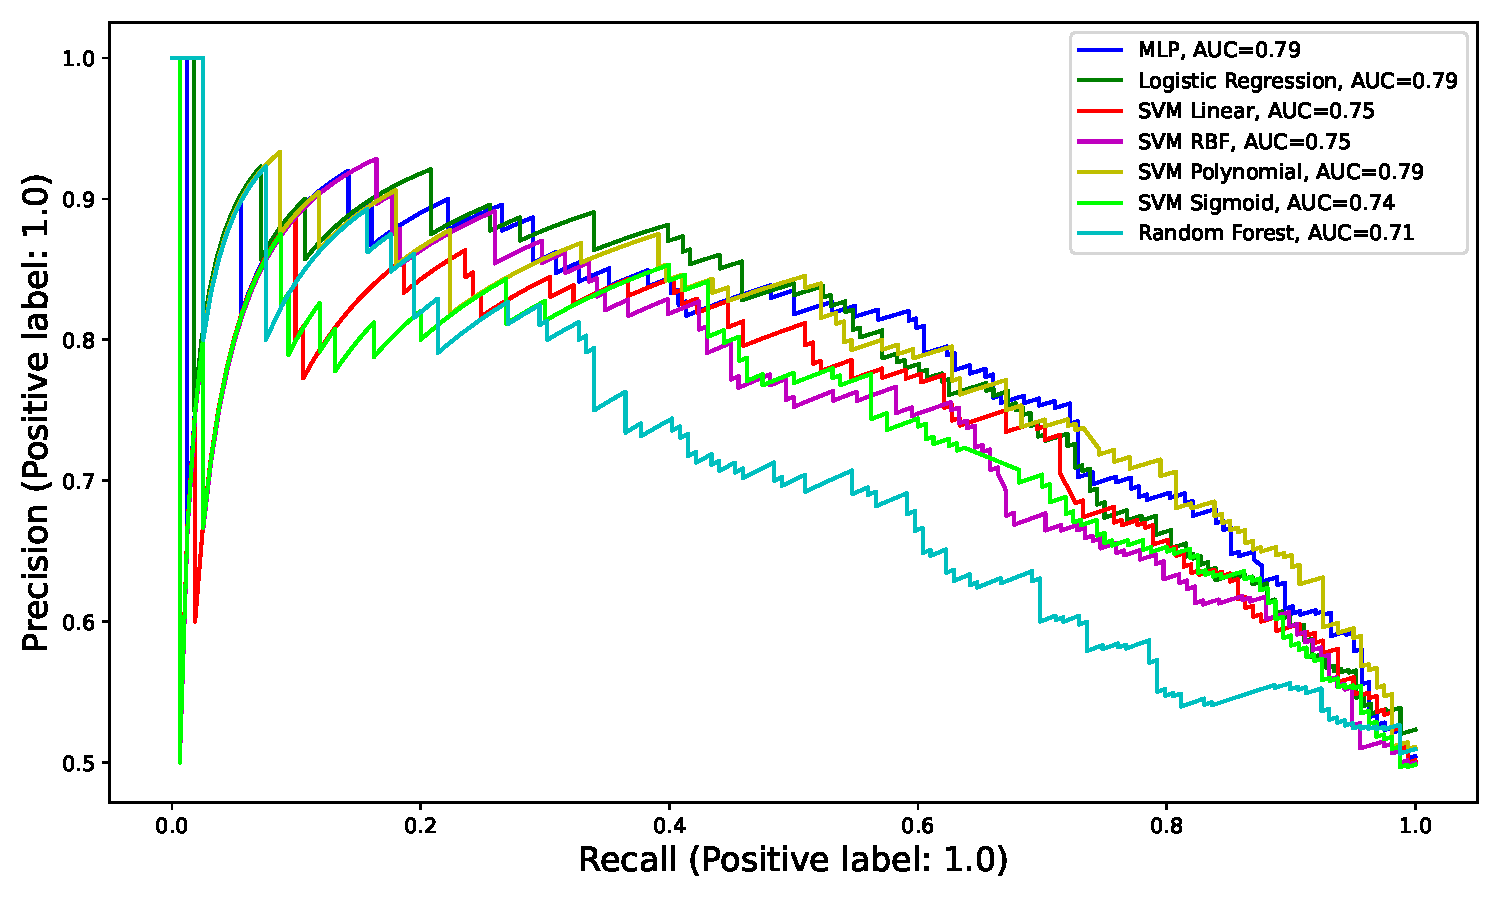
\includegraphics[width=8.5cm]{plots/parcurve.pdf}
\caption{Precision and Recall Curves.}
%\denes{As discussed, please replot without axis / bigger fonts or single plot}}

\label{fig:par}
\centering
\end{figure}

